\documentclass[]{beamer}
\usetheme{Boadilla}
\usepackage{tikz}
\usetikzlibrary{positioning}
\usetikzlibrary{shapes.multipart}
%\usepackage{minted}
\usepackage{fancyvrb}
\usepackage[utf8]{inputenc}
\usepackage{graphicx}
\usepackage{xcolor}
\usepackage{listings}
\usepackage{tabulary}
\usepackage{colortbl}
		
%New colors defined below
\definecolor{codegreen}{rgb}{0,0.6,0}
\definecolor{codegray}{rgb}{0.5,0.5,0.5}
\definecolor{codepurple}{rgb}{0.58,0,0.82}
\definecolor{backcolour}{RGB}{240,240,240}

%Code listing style named "mystyle"
\lstdefinestyle{mystyle}{
  backgroundcolor=\color{backcolour},   commentstyle=\color{codegreen},
  keywordstyle=\color{blue},
  numberstyle=\tiny\color{codegray},
  stringstyle=\color{orange},
  basicstyle=\ttfamily\footnotesize,
  breakatwhitespace=false,         
  breaklines=true,                 
  captionpos=b,                    
  keepspaces=true,                 
  numbers=none,                    
  numbersep=5pt,                  
  showspaces=false,                
  showstringspaces=false,
  showtabs=false,                  
  tabsize=2
}
 
\lstset{style=mystyle}
   
\renewcommand{\vec}[1]{\boldsymbol{#1}}
\newcommand{\ques}{\textbf{\textcolor{red}{Question:  }}}
\newcommand{\questionssofar}{\begin{frame}\frametitle{Any questions?}\end{frame}}

\title[BERT (\& the Sesame Street)]{Chapter 10: \\ BERT (\& the Sesame Street)}
\author{Matthias Aßenmacher}
\date{January 20, 2021}

\begin{document}
\begin{frame}
\titlepage
\end{frame}



\begin{frame}{Key facts of BERT \href{https://arxiv.org/pdf/1810.04805.pdf}{\beamergotobutton{Devlin et al. (2018)}}}

\begin{figure}
\centering

\includegraphics[width = 3cm]{figure/bert.jpeg}
\end{figure}

\textit{\textbf{B}idirectional \textbf{E}ncoder \textbf{R}epresentations from \textbf{T}ransformers:}
\begin{itemize}
		\item Bidirectionally contextual model
		\item Introduces new self-supervised objective(s)
		\item Completely replaces recurrent architectures by Self-Attention\\$+$ simultaneously able to include bidirectionality
\end{itemize}
\end{frame}



\begin{frame}{Predecessors of BERT}
\hbox{\hspace{-4.5em} 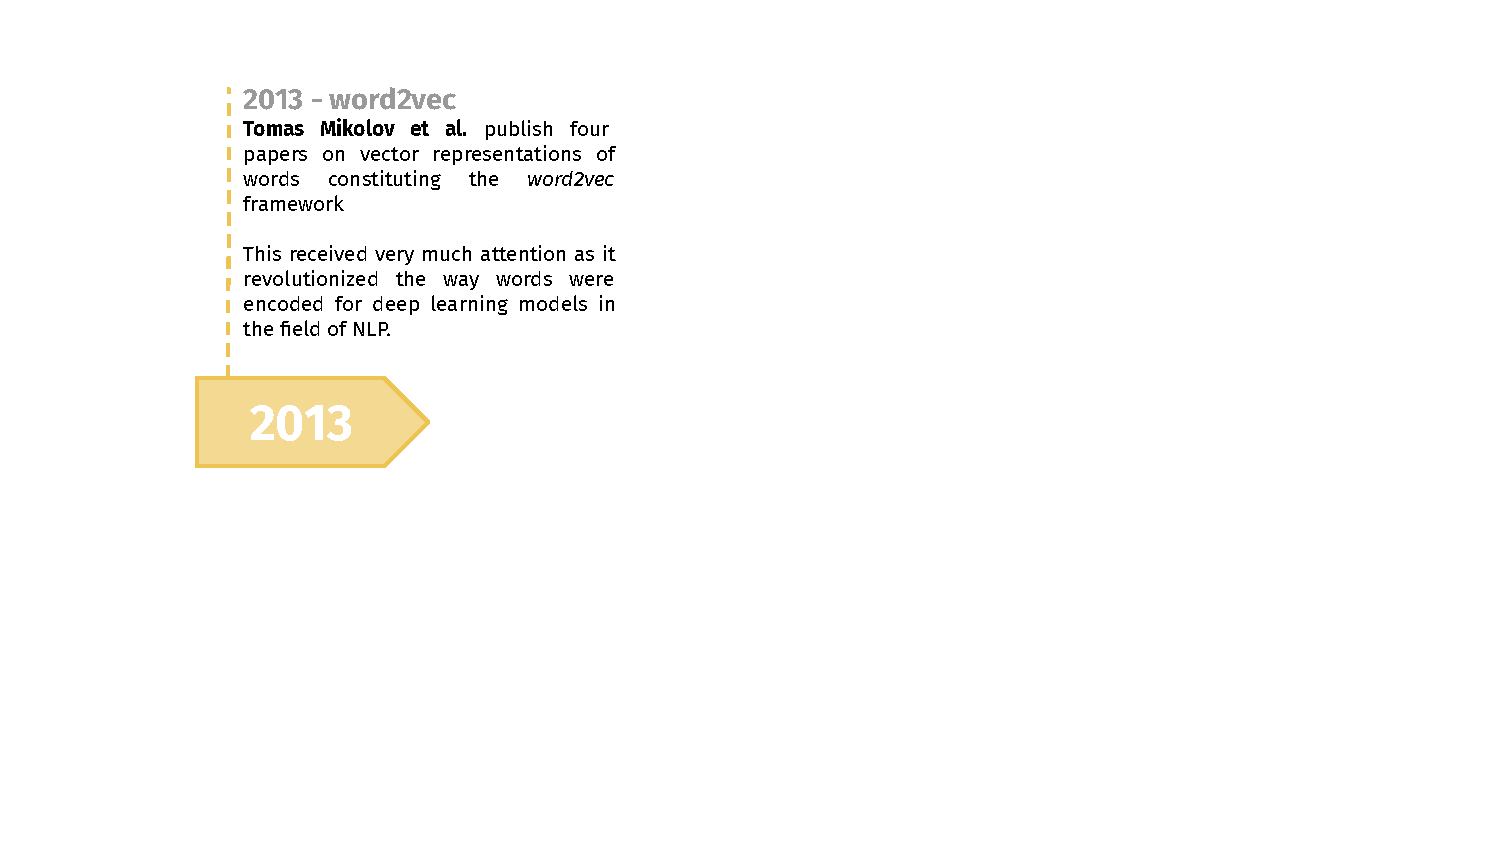
\includegraphics[width=14cm,page=1]{figure/transfer_learning_timeline1_nlp.pdf}}
\end{frame}
\begin{frame}[noframenumbering]{Predecessors of BERT}
\hbox{\hspace{-4.5em} \includegraphics[width=14cm,page=2]{figure/transfer_learning_timeline1_nlp.pdf}}
\end{frame}
\begin{frame}[noframenumbering]{Predecessors of BERT}
\hbox{\hspace{-4.5em} \includegraphics[width=14cm,page=3]{figure/transfer_learning_timeline1_nlp.pdf}}
\end{frame}
\begin{frame}[noframenumbering]{Predecessors of BERT}
\hbox{\hspace{-4.5em} \includegraphics[width=14cm,page=4]{figure/transfer_learning_timeline1_nlp.pdf}}
\end{frame}
\begin{frame}[noframenumbering]{Predecessors of BERT}
\hbox{\hspace{-4.5em} \includegraphics[width=14cm,page=5]{figure/transfer_learning_timeline1_nlp.pdf}}
\end{frame}



\begin{frame}{Core of BERT \href{https://arxiv.org/pdf/1810.04805.pdf}{\beamergotobutton{Devlin et al. (2018)}}}
\begin{figure}
\centering
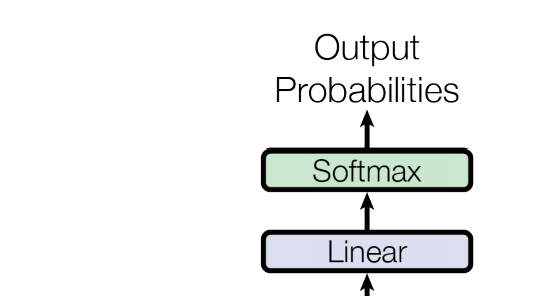
\includegraphics[width = 3.2cm]{figure/bert-top.png}\\ 
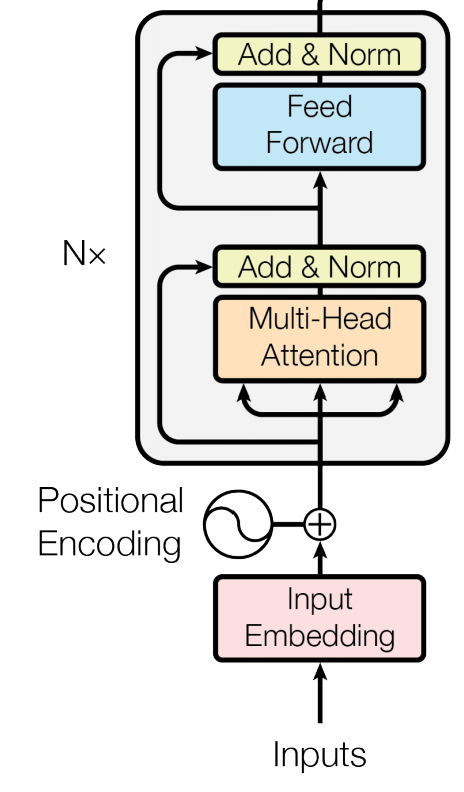
\includegraphics[width = 3cm]{figure/bert-bottom.png}\\ 
\footnotesize{Source:} \href{https://arxiv.org/pdf/1706.03762.pdf}{\beamergotobutton{Vaswani et al. (2017)}}
\end{figure}
\end{frame}



\begin{frame}{A remark on Self-Supervision}
	\textbf{Causality is an issue!}
	
	\begin{itemize}
		\item \textit{Remember:} Input and target sequences are the same\\
					$\rightarrow$ We modify the input to create a meaningful task 
		\item A sequence is used to predict itself again
		\item Bidirectionality at a lower layer would allow a word to see itself at later hidden layers\\
					$\rightarrow$ The model would be allowed to cheat!\\
					$\rightarrow$ This would not lead to meaningful internal representations
	\end{itemize}
\end{frame}



\begin{frame}{GPT vs. ELMo vs. BERT}

\begin{figure}
\centering
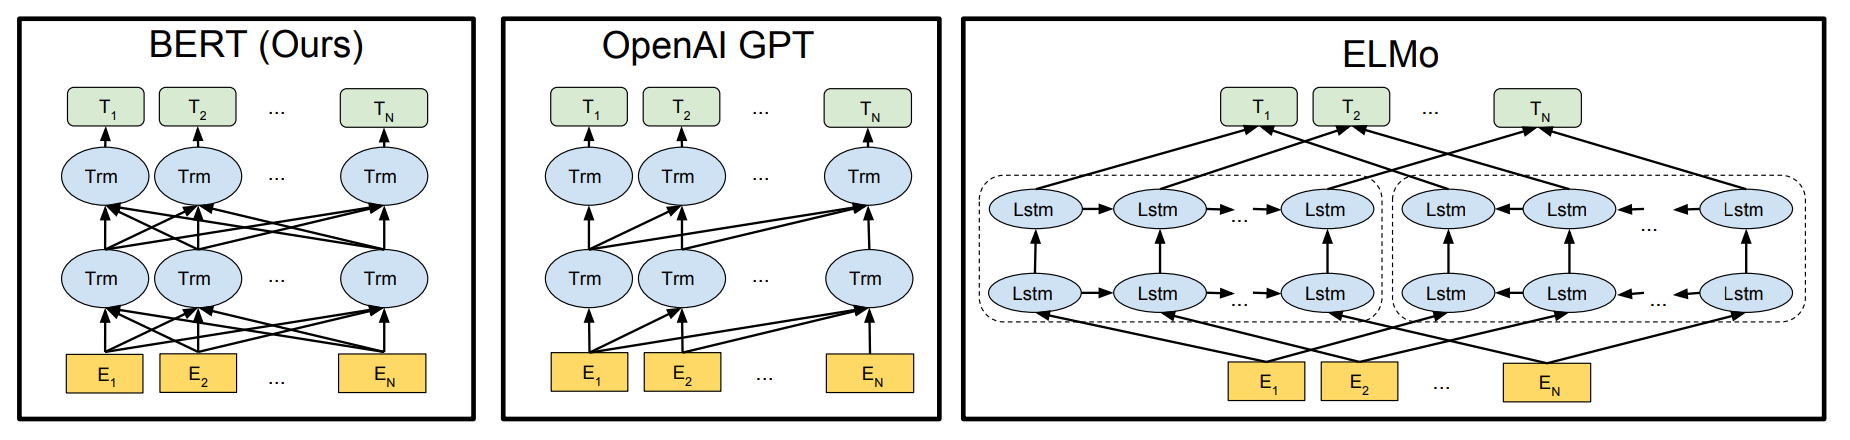
\includegraphics[width = 11cm]{figure/comparison-bert.png}\\ 
\footnotesize{Source:} \href{https://arxiv.org/pdf/1810.04805.pdf}{\beamergotobutton{Devlin et al. (2018)}}
\end{figure}

\textbf{Major architectural differences:}

\begin{itemize}
\item ELMo uses two separate unidirectional models to achieve bidirectionality\\
  $\rightarrow$ Only "\textit{shallow}" bidirectionality
\item GPT is not bidirectional, thus no issues concerning causality
\item BERT combines the best of both worlds: $$Self\text{-}Attention + (Deep)\;Bidirectionality$$
\end{itemize} 
\end{frame}



\begin{frame}{Masked Language Modeling (MLM)}

\textbf{First of all:}

\begin{itemize}
\item It has nothing to do with Masked Self-Attenion\\ 
  $\rightarrow$ Masked Self-Attention is an architectural detail in the decoder of a Transformer, i.e. used by e.g. GPT
\item Masked Self-Attention as a way to induce causality in the decoder
\item MLM is a modeling objective introduced to couple Self-Attention and (deep) bidirectionality without violating causality
\end{itemize}
\end{frame}



\begin{frame}{Masked Language Modeling (MLM) ctd.}

\textbf{Masked Language Modeling:}

\begin{itemize}
\item \textbf{Training objective:} $$\text{Given a sentence, predict \texttt{[MASK]}ed tokens}$$
\item \textbf{Generation of samples:} $$\text{Randomly replace* a fraction of the words by \texttt{[MASK]}}$$
  \scriptsize *Sample 15\% of the tokens; replace 80\% of them by \texttt{[MASK]}, 10\% by a random token \& leave 10\% unchanged
\item \normalsize \textbf{Input:}\\\mbox{}\\
			\footnotesize
\begin{tabular}{|cccccccccc|}
\hline
The & quick & brown & \cellcolor{blue!65}\texttt{[MASK]} & jumps & over & the & \cellcolor{blue!65}\texttt{[MASK]} & dog & . \\
\hline
\end{tabular}\\\mbox{}
\item \normalsize \textbf{Targets:} $$(fox,\; lazy)$$
\end{itemize}
\end{frame}



\begin{frame}{Masked Language Modeling (MLM) ctd.}

\textbf{Discrepancy between pre-training \& fine-tuning:}

	\begin{itemize}
		\item \texttt{[MASK]}-token as central part of pre-training procedure
		\item \texttt{[MASK]}-token does not occur during fine-tuning
		\item \textbf{Modified pre-training task:}\\
					Predict 15\% of the tokens of which only 80\% have been replaced by \texttt{[MASK]}
					\begin{itemize}
						\item 80\% of the selected tokens:\\
									\texttt{The quick brown fox $\rightarrow$ The quick brown [MASK]}
						\item 10\% of the selected tokens:\\
									\texttt{The quick brown fox $\rightarrow$ The quick brown went}
						\item 10\% of the selected tokens:\\
									\texttt{The quick brown fox $\rightarrow$ The quick brown fox}
					\end{itemize}
	\end{itemize}
\end{frame}



\begin{frame}{Next Sentence Prediction (NSP)}

\textbf{Next Sentence Prediction:}

\begin{itemize}
\item \textbf{Training objective:} $$\text{Given two sentences, predict whether $s_2$ follows $s_1$}$$
\item \textbf{Generation of samples:} $$\text{Randomly sample* negative examples (cf. word2vec)}$$
  \scriptsize *50\% of the time the second sentence is the actual next sentence, 50\% of the time it is a randomly sampled sentence
\item \normalsize \textbf{Full Input:}\\\mbox{}\\
			\footnotesize
\begin{center}
\begin{tabular}{|cccccccc|}
\hline
\cellcolor{blue!15}\texttt{[CLS]} & The & \cellcolor{blue!65}\texttt{[MASK]} & is & quick & . & \cellcolor{blue!15}\texttt{[SEP]} &\\\hline\hline It & jumps & over & the & \cellcolor{blue!65}\texttt{[MASK]} & dog & . & \cellcolor{blue!15}\texttt{[SEP]} \\
\hline
\end{tabular}\\\mbox{}
\end{center}
\item \normalsize \texttt{[CLS]} token as sequence representation for classification
\item \texttt{[SEP]} token for separation of the two input sequences
\end{itemize}
\end{frame}



\begin{frame}{BERT's input embeddings}
\begin{figure}
\centering
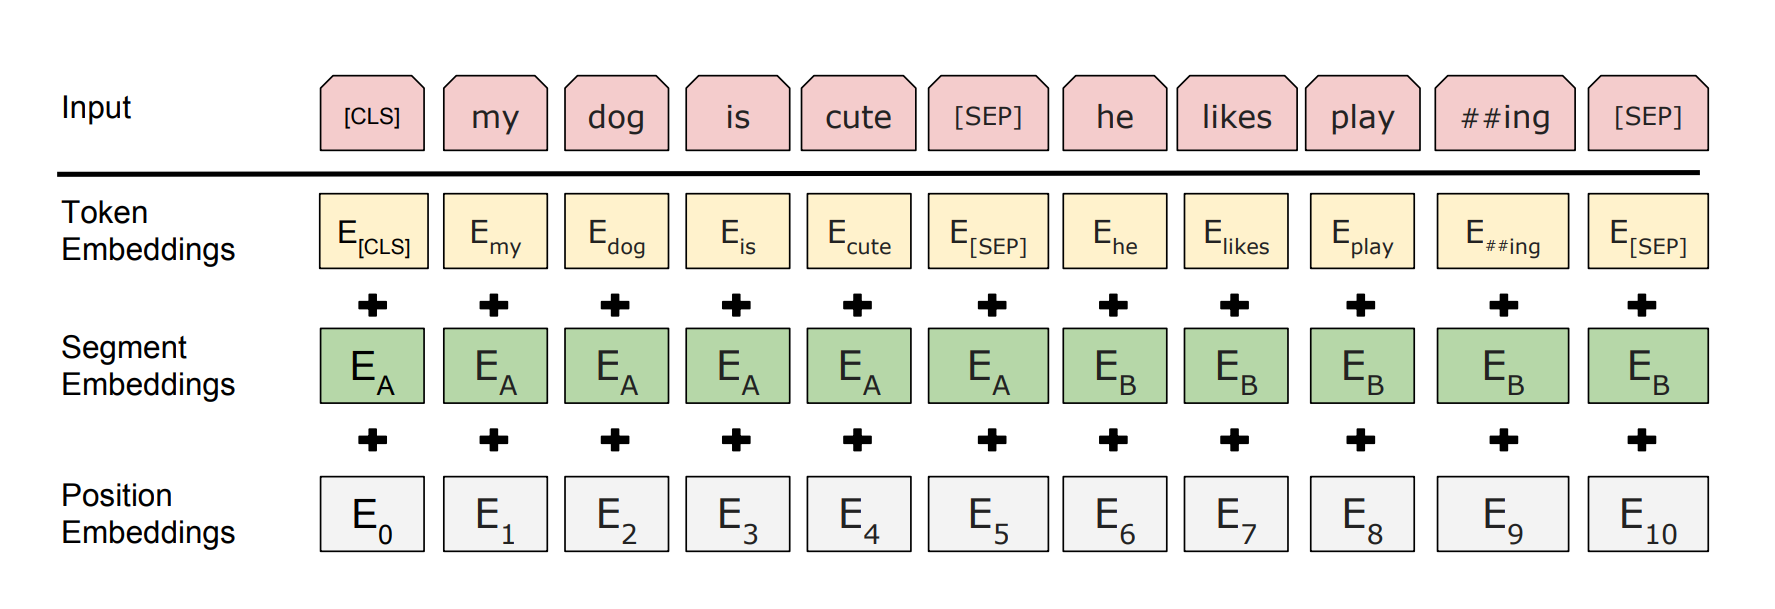
\includegraphics[width = 12cm]{figure/bert-input.png}\\ 
\footnotesize{Source:} \href{https://arxiv.org/pdf/1810.04805.pdf}{\beamergotobutton{Devlin et al. (2018)}}
\end{figure}

	\begin{itemize}
		\item Byte-Pair encoding \href{https://www.aclweb.org/anthology/P16-1162.pdf}{\beamergotobutton{Sennrich et al. (2016)}} for the inputs\\
				$\rightarrow$ Vocabulary of 30.000 tokens
	\end{itemize}
\end{frame}



\begin{frame}{Pre-Training BERT}

\textbf{Ingredients:}

\begin{itemize}
	\item Massive lexical resources (BooksCorpus $+$ Eng. Wikipedia)\\
				$\rightarrow$ 13 GB in total
	\item Train for approximately* 40 epochs
	\item 4 (16) \href{https://cloud.google.com/tpu/}{Cloud TPUs} for 4 days for the BASE (LARGE) variant
	\item 12 (24) Transformer encoder blocks with an embedding size of $E = 768$ (1024) and a hidden layer size $H = E$, $H/64 = 12$ (16) attention heads are used and the feed-forward size is set to $4H$\\
				$\rightarrow$ 110M (340M) model parameters in total for $BERT_{Base}$ ($BERT_{Large}$)
	\item Loss function: $$Loss_{BERT} = Loss_{MLM} + Loss_{NSP}$$
\end{itemize}
				\vspace{.3cm}
				{\scriptsize *1.000.000 steps on batches of 256 sequences with a sequence length of 512 tokens}
\end{frame}



\begin{frame}{Pre-Training BERT -- Maximum sequence length}

\begin{figure}
\centering
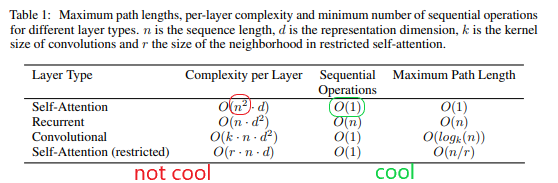
\includegraphics[width = 8.5cm]{figure/bert-problem.png}\\ 
\footnotesize{Source:} \href{https://arxiv.org/pdf/1706.03762.pdf}{\footnotesize Vaswani et al. (2017)}
\end{figure}

\textbf{Limitation:}

\begin{itemize}
	\item BERT can only consume sequences of up to 512 tokens
	\item Two sentences for NSP are sampled such that $$length_{sentence A} + length_{sentence B} \leq 512$$
	\item Reason: Computational complexity of Transformer scales quadratically with the sequence length\\
				$\rightarrow$ Longer sequences are disproportionally expensive
\end{itemize}
\end{frame}



\begin{frame}{Fine-Tuning BERT}
\begin{figure}
\centering
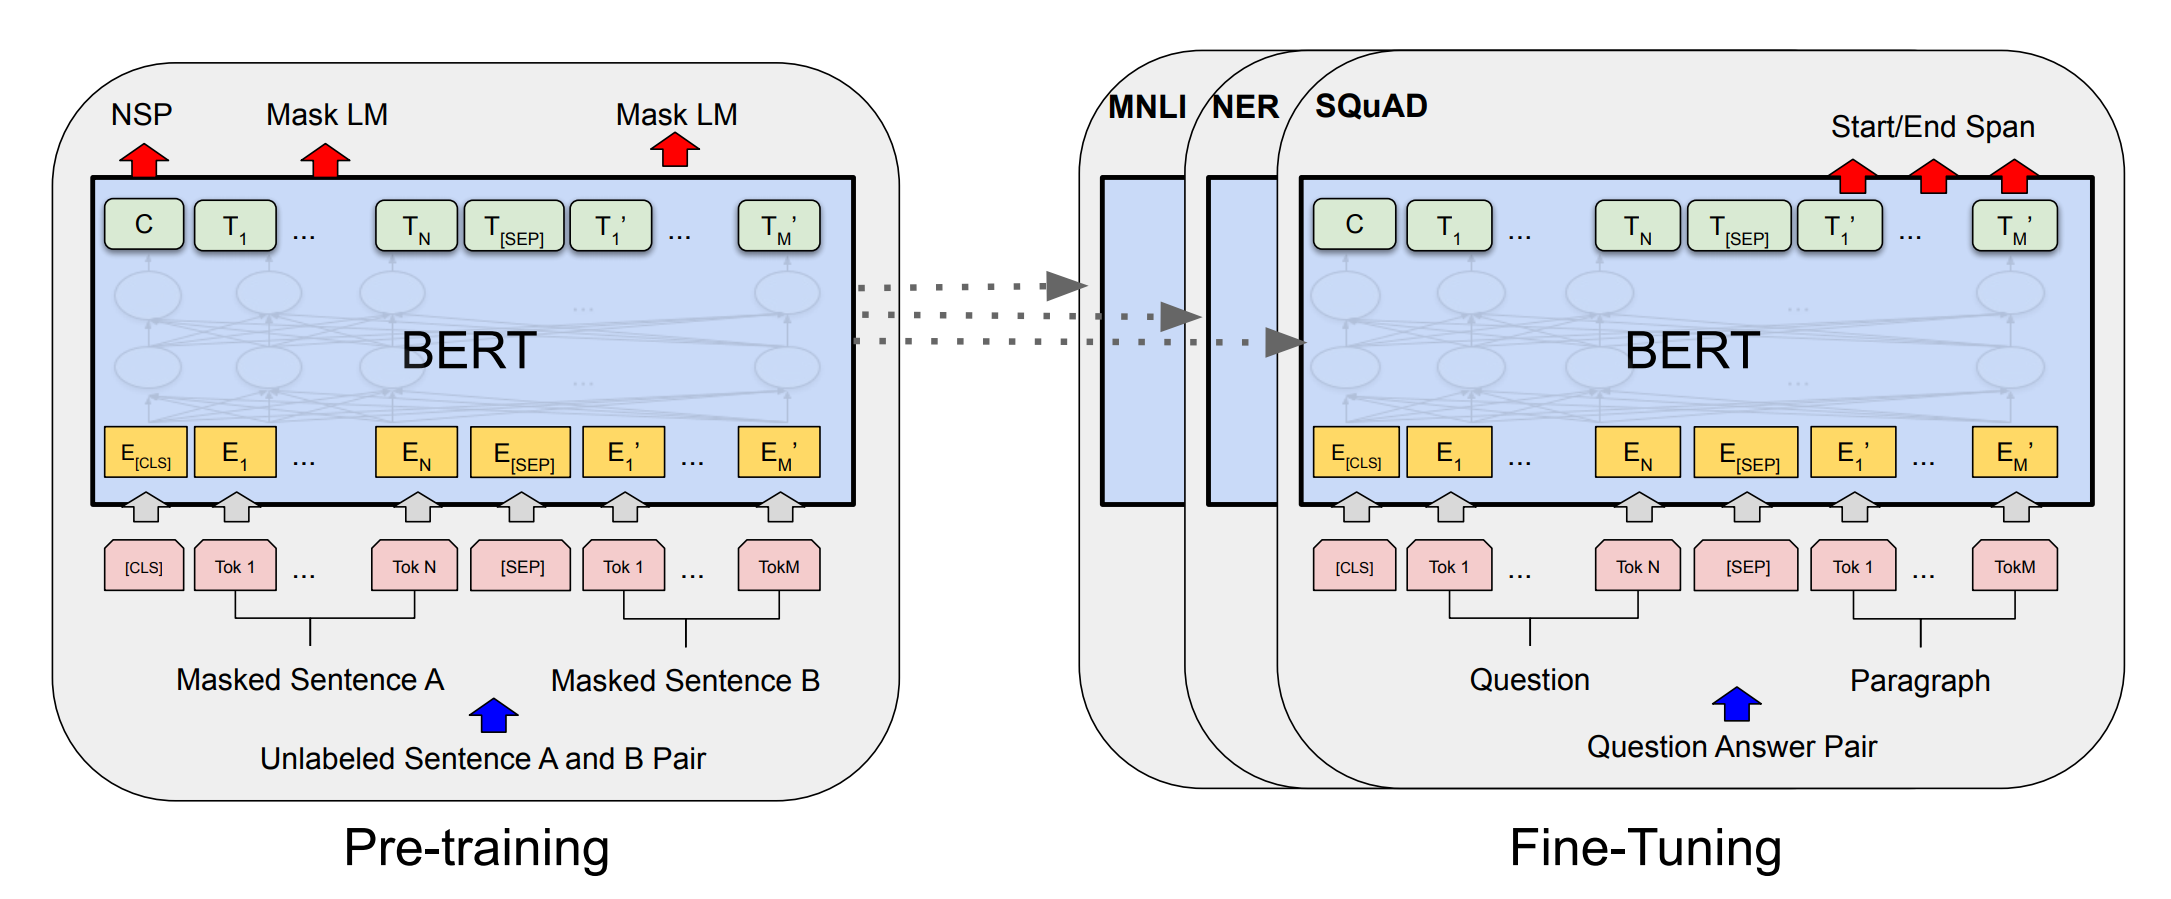
\includegraphics[width = 11cm]{figure/bert-tasks.png}\\ 
\footnotesize{Source:} \href{https://arxiv.org/pdf/1810.04805.pdf}{\footnotesize Devlin et al. (2018)}
\end{figure}
\end{frame}



\begin{frame}{Fine-Tuning BERT} \label{bert-glue}
\begin{figure}
\centering
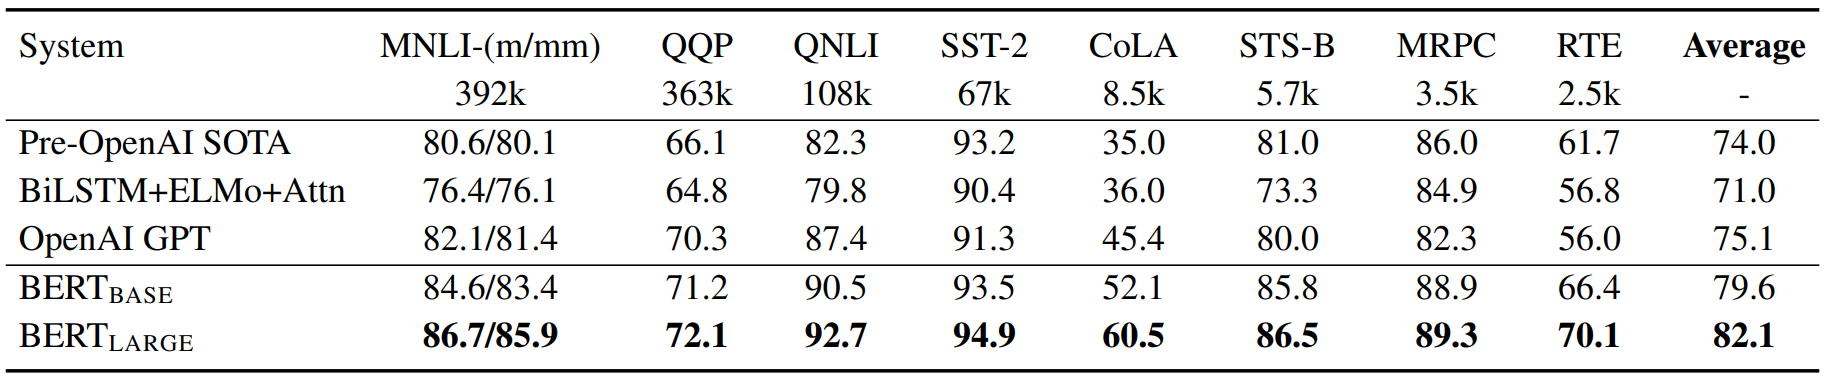
\includegraphics[width = 11cm]{figure/bert-sota.png}\\ 
\footnotesize{Source:} \href{https://arxiv.org/pdf/1810.04805.pdf}{\footnotesize Devlin et al. (2018)}
\end{figure}
\begin{itemize}
	\item Performance of BERT on the \href{https://gluebenchmark.com/}{\beamergotobutton{GLUE Benchmark}}
	\item Beats all of the previous state-of-the-art models
	\item In the meantime: Other models better than BERT
\end{itemize}
\end{frame}



\begin{frame}{Successors of BERT}
\hbox{\hspace{-4.5em} 
\includegraphics[width=14cm,page=1]{figure/transfer_learning_timeline2_nlp.pdf}}
\end{frame}
\begin{frame}[noframenumbering]{Successors of BERT}
\hbox{\hspace{-4.5em} 
\includegraphics[width=14cm,page=2]{figure/transfer_learning_timeline2_nlp.pdf}}
\end{frame}
\begin{frame}[noframenumbering]{Successors of BERT}
\hbox{\hspace{-4.5em} 
\includegraphics[width=14cm,page=3]{figure/transfer_learning_timeline2_nlp.pdf}}
\end{frame}
\begin{frame}[noframenumbering]{Successors of BERT}
\hbox{\hspace{-4.5em} 
\includegraphics[width=14cm,page=4]{figure/transfer_learning_timeline2_nlp.pdf}}
\end{frame}
\begin{frame}[noframenumbering]{Successors of BERT}
\hbox{\hspace{-4.5em} 
\includegraphics[width=14cm,page=5]{figure/transfer_learning_timeline2_nlp.pdf}}
\end{frame}



\begin{frame}{BERTology \href{https://arxiv.org/pdf/2002.12327.pdf}{\beamergotobutton{Rodgers et al., 2020}}}\label{bert-lit}

\textbf{Post-BERT architectures:}

\begin{itemize}
\item Most architectures still rely on either an encoder- \textit{or} a decoder-style type of model (e.g. \href{https://cdn.openai.com/better-language-models/language_models_are_unsupervised_multitask_learners.pdf}{\beamergotobutton{GPT2}}, \href{https://arxiv.org/pdf/1906.08237.pdf}{\beamergotobutton{XLNet}})
\item \textit{BERTology:} Many papers/models which aim at ..
			\begin{itemize}
				\item .. explanining BERT (e.g. \href{https://arxiv.org/pdf/1906.02715.pdf}{\beamergotobutton{Coenen et al., 2019}}, \href{https://arxiv.org/pdf/1905.10650.pdf}{\beamergotobutton{Michel et al., 2019}})
				\item .. improving BERT (\href{https://arxiv.org/pdf/1907.11692.pdf}{\beamergotobutton{RoBERTa}}, \href{https://arxiv.org/pdf/1909.11942.pdf}{\beamergotobutton{ALBERT}})
				\item .. making BERT more efficient (\href{https://arxiv.org/pdf/1909.11942.pdf}{\beamergotobutton{ALBERT}}, \href{https://arxiv.org/pdf/1910.01108.pdf}{\beamergotobutton{DistilBERT}})
				\item .. modifying BERT (\href{https://arxiv.org/pdf/1910.13461.pdf}{\beamergotobutton{BART}})
			\end{itemize}
\item Overview on many different papers:\\
			\href{https://github.com/tomohideshibata/BERT-related-papers}{https://github.com/tomohideshibata/BERT-related-papers}
\end{itemize}
\end{frame}



\begin{frame}{RoBERTa \href{https://arxiv.org/pdf/1907.11692.pdf}{\beamergotobutton{Liu et al., 2019}}}

	\textbf{Improvements in Pre-Training:}

	\begin{itemize}
		\item Authors claim that BERT is seriously undertrained
		\item Change of the \texttt{MASK}ing strategy  \\
					$\rightarrow$ BERT masks the sequences once before pre-training  \\
					$\rightarrow$ RoBERTa uses dynamic \texttt{MASK}ing  \\
					$\Rightarrow$ RoBERTa sees the same sequence \texttt{MASK}ed differently
		\item RoBERTa does not use the additional NSP objective during pre-training
		\item 160 GB of pre-training resources instead of 13 GB
		\item Pre-training is performed with larger batch sizes (8k)
	\end{itemize}
\end{frame}



\begin{frame}{Dynamic vs. Static Masking \href{https://arxiv.org/pdf/1907.11692.pdf}{\beamergotobutton{Liu et al., 2019}}}

	\textbf{Static Masking (BERT):}

	\begin{itemize}
		\item Apply \texttt{MASK}ing procedure to pre-training corpus once
		\item (additional for BERT: Modify the corpus for NSP)
		\item Train for approximately 40 epochs
	\end{itemize}

\vspace{.3cm}

	\textbf{Dynamic Masking (RoBERTa):}

	\begin{itemize}
		\item Duplicate the training corpus \textit{ten} times
		\item Apply \texttt{MASK}ing procedure to each duplicate of the pre-training corpus
		\item Train for 40 epochs
		\item Model sees each training instance in ten different "versions"\\
					(each version four times) during pre-training
	\end{itemize}
\end{frame}



\begin{frame}{RoBERTa \href{https://arxiv.org/pdf/1907.11692.pdf}{\beamergotobutton{Liu et al., 2019}}}

\textbf{Architectural differences:}

\begin{itemize}
\item Architecture (layers, heads, embedding size) identical to BERT
\item 50k token BPE vocabulary instead of 30k
\item Model size differs (due to the larger embedding matrix)\\
			$\Rightarrow$ $\sim$ 125M (360M) for the BASE (LARGE) variant 
\end{itemize}

\textbf{Performance differences:}

\begin{figure}
\centering
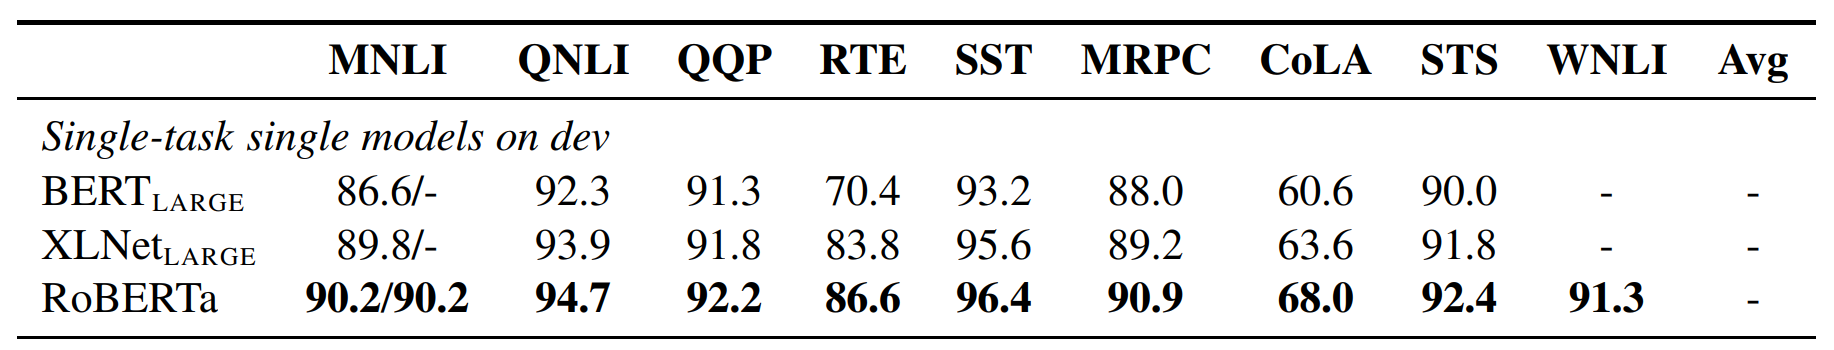
\includegraphics[width = 11cm]{figure/roberta-sota.png}\\ 
\footnotesize{Source:} \href{https://arxiv.org/pdf/1907.11692.pdf}{\footnotesize Liu et al. (2019)}
\end{figure}
\footnotesize
\textit{Note:} Liu et al. (2019) report the accuracy for QQP while Devlin et al. (2018) report the F1 score (cf. results displayed on slide \ref{bert-glue}); XLNet: see next Chapter.
\end{frame}



\begin{frame}{ALBERT \href{https://arxiv.org/pdf/1909.11942.pdf}{\beamergotobutton{Lan et al., 2019}}}

	\textbf{Changes in the architecture:}

	\begin{itemize}
		\item Disentanglement of embedding size $E$ and hidden layer size $H$\\
					$\rightarrow$ WordPiece-Embeddings (size $E$) context-independent\\
					$\rightarrow$ Hidden-Layer-Embeddings (size $H$) context-dependent\\
					$\Rightarrow$ Setting $H >> E$ enlargens model capacity without increasing the size of the embedding matrix,\\
					since $O(V \times H) > O(V \times E +  E \times H)$ if $H >> E$.
		\item Cross-Layer parameter sharing
		\item Change of the pre-training NSP loss\\
					$\rightarrow$ Introduction of \textit{Sentence-Order Prediction} (SOP)\\
					$\rightarrow$ Positive examples created alike to those from NSP\\
					$\rightarrow$ Negative examples: Just swap the ordering of sentences
		\item $n-gram$ masking for the MLM task
\end{itemize}
\end{frame}



\begin{frame}{ALBERT \href{https://arxiv.org/pdf/1909.11942.pdf}{\beamergotobutton{Lan et al., 2019}}}

	\textbf{Performance differences:}

	\begin{figure}
		\centering
		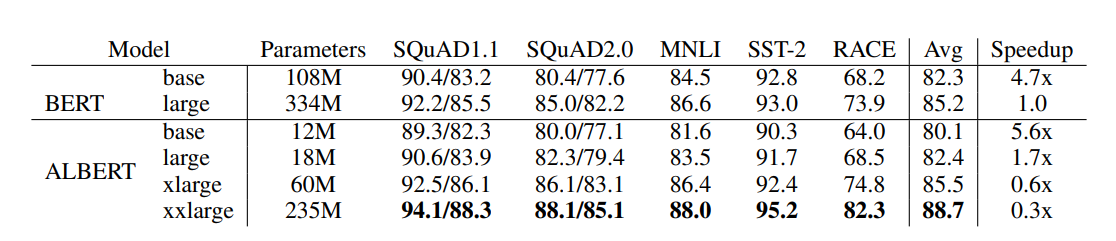
\includegraphics[width = 11cm]{figure/albert-sota.png}\\ 
		\footnotesize{Source:} \href{https://arxiv.org/pdf/1907.11942.pdf}{\footnotesize Lan et al. (2019)}
	\end{figure}

	\textbf{Notes:}

	\begin{itemize}
		\item In General: Smaller model size (because of parameter sharing)
		\item Nevertheless: Scale model up to almost similar size (\texttt{xxlarge} version)
		\item Strong performance compared to BERT
	\end{itemize}
\end{frame}


\begin{frame}{Using BERT \& Co.}

\textbf{Native implementations:}

		\begin{itemize}
			\item BERT: \href{https://github.com/google-research/bert}{\textit{https://github.com/google-research/bert}}
			\item RoBERTa: \small\href{https://github.com/pytorch/fairseq/tree/master/examples/roberta}{\textit{https://github.com/pytorch/fairseq/tree/master/examples/roberta}}\normalsize
			\item ALBERT: \href{https://github.com/google-research/ALBERT}{\textit{https://github.com/google-research/ALBERT}}\normalsize
		\end{itemize}

\vspace{.3cm}

\textbf{Drawbacks:}

		\begin{itemize}
			\item Different frameworks use for the implementations
			\item Different programming styles\\
						$\rightarrow$ Adaption of different models to custom problems can sometimes lead to a lot of redundant work
		\end{itemize}
\end{frame}



\begin{frame}[fragile]{Example: Fine-tune native BERT on MRPC}

\textbf{Command line:}
\vspace{-.2cm}
\begin{lstlisting}[language=Python]
	!python run_classifier.py \
  --task_name=MRPC \
  --do_train=true \
  --do_eval=true \
  --data_dir=$GLUE_DIR/MRPC \
  --vocab_file=$BERT_BASE_DIR/vocab.txt \
  --bert_config_file=$BERT_BASE_DIR/bert_config.json \
  --init_checkpoint=$BERT_BASE_DIR/bert_model.ckpt \
  --max_seq_length=128 \
  --train_batch_size=32 \
  --learning_rate=2e-5 \
  --num_train_epochs=3.0 \
  --output_dir=/tmp/mrpc_output/
\end{lstlisting}
\end{frame}



\begin{frame}{Pre-trained architectures @ \href{https://github.com/huggingface/transformers}{\texttt{transformers}}}

\textbf{Unified API for state-of-the-art architectures:}

\begin{itemize}
	\item 32+ pre-trained architectures (as of \today)
	\item Models in 100+ languages available (as of \today)
	\item Implementations in PyTorch as well as TensorFlow 2.0
	\item Unified naming model parts and fine-tuning procedures
	\item Docs: \href{https://huggingface.co/transformers/index.html}{\textit{https://huggingface.co/transformers/index.html}}
\end{itemize}

\vspace{.3cm}

\textbf{Which different building blocks available?}

\begin{itemize}
	\item Model architecture
	\item Custom tokenizers for each architecture
	\item (Sets of) Pre-trained weights for an architecture
	\item Pre-defined heads for fine-tuning on common tasks
\end{itemize}
\end{frame}



\begin{frame}[fragile]{Pre-trained architectures @ \href{https://github.com/huggingface/transformers}{\texttt{transformers}}}

\textbf{Pre-trained weights:}
\vspace{-.2cm}
\begin{lstlisting}[language=Python]
<model name>-<version>-<cased/uncased>
\end{lstlisting}

\vspace{.3cm}

\textbf{Load tokenizer \& tokenize a sentence:}
\vspace{-.2cm}
\begin{lstlisting}[language=Python]
from transformers import BertTokenizer
tokenizer = BertTokenizer.from_pretrained("bert-base-cased")
sentence = "Hello guys, welcome to the course."

ids = tokenizer.encode(sentence, add_special_tokens = True)
ids

# [101, 8667, 3713, 117, 7236, 1106, 1103, 1736, 119, 102]

[tokenizer.convert_ids_to_tokens(id) for id in ids]

# ['[CLS]', 'Hello', 'guys', ',', 'welcome', 'to', 'the', 
#  'course', '.', '[SEP]']
\end{lstlisting}
\end{frame}



\begin{frame}[fragile]{Pre-trained architectures @ \href{https://github.com/huggingface/transformers}{\texttt{transformers}}}

\textbf{Tokenization all in one:}

\begin{itemize}
		\item BERT requires inputs of fixed length $\rightarrow$ Padding
		\item \texttt{[PAD]} tokens should not receive Attention weights
\end{itemize}
\vspace{-.2cm}
\begin{lstlisting}[language=Python]
tokenizer.encode_plus(sentence, 
                      add_special_tokens = True,
                      max_length = 12,          
                      pad_to_max_length = True,
                      return_attention_mask = True,   
                      return_tensors = 'pt'
                   )
                   
# {'input_ids': tensor([[ 101, 8667, 3713,  117, 7236, 
#                      1106, 1103, 1736,  119,  102,    0,    0]]),
# 'token_type_ids': tensor([[0, 0, 0, 0, 0, 0, 0, 0, 0, 0, 0, 0]]),
# 'attention_mask': tensor([[1, 1, 1, 1, 1, 1, 1, 1, 1, 1, 0, 0]])}
\end{lstlisting}
\end{frame}



\begin{frame}[fragile]{Pre-trained architectures @ \href{https://github.com/huggingface/transformers}{\texttt{transformers}}}

\textbf{Load a model architecture:}
\vspace{-.2cm}
\begin{lstlisting}[language=Python]
from transformers import BertForSequenceClassification
mod = BertForSequenceClassification.from_pretrained("bert-base-cased",
                                                    num_labels = 3)
\end{lstlisting}

\vspace{.3cm}

\textbf{Inspect the dimensionality of the model:}
\vspace{-.2cm}
\begin{lstlisting}[language=Python]
params = list(mod.parameters())

## size of the embedding layer
params[0].shape

# torch.Size([28996, 768])

## size of the classification layer
params[200].shape

# torch.Size([3])
\end{lstlisting}
\end{frame}



\begin{frame}[fragile]{Pre-trained architectures @ \href{https://github.com/huggingface/transformers}{\texttt{transformers}}}

\textbf{Pipelines:}

\begin{itemize}
		\item Extremely high-level API included in \texttt{transformers}
		\item Available for a couple of different downstream tasks
		\item Ingredients of a pipeline: 
		\begin{itemize}
				\item \textit{Encoding:} Tokenization of the inputs 
				\item Inferency by a chosen model
				\item \textit{Decoding:} Use model output to generate target values
		\end{itemize}
\end{itemize}
\vspace{-.2cm}
\begin{lstlisting}[language=Python]
from transformers import pipeline

pipeline(<task name>, model = <model name>, 
         tokenizer = <tokenizer name>)
\end{lstlisting}

\begin{itemize}
		\item \texttt{model} and \texttt{tokenizer} are optional arguments\\
  $\rightarrow$ If not provided, some internal defaults are used
\end{itemize}
\end{frame}


\begin{frame}[fragile]{Pre-trained architectures @ \href{https://github.com/huggingface/transformers}{\texttt{transformers}}}

\textbf{Available tasks (as of \today):}

\begin{itemize}
		\item Feature Extraction (\texttt{feature-extraction})
		\item Sentiment Analysis (\texttt{"sentiment-analysis"})
		\item Named entity recognition (\texttt{"ner"})
		\item Question Answering (\texttt{"question-answering"})
		\item \texttt[MASK]-filling (\texttt{"fill-mask"})
		\item Summarization (\texttt{"summarization"})
		\item Translation (\texttt{"translation-xx-to-yy"})
		\item seq2seq Text Generation (\texttt{"text2text-generation"})
		\item Text Generation (\texttt{"text-generation"})
		\item Zero-Shot Classification (\texttt{"zero-shot-classification"})
		\item Multi-turn Conversation (\texttt{"conversation"})
\end{itemize}
\end{frame}



\begin{frame}[fragile]{Pre-trained architectures @ \href{https://github.com/huggingface/transformers}{\texttt{transformers}}}

\textbf{Exemplary task (with default model):}
\vspace{-.2cm}
\begin{lstlisting}[language=Python]
from transformers import pipeline

pipe_classif = pipeline("sentiment-analysis")
pipe_classif(sentence)

# [{'label': 'POSITIVE', 'score': 0.99960136}]

pipe_classif("I absolutely hate this!")

# [{'label': 'NEGATIVE', 'score': 0.9992645}]
\end{lstlisting}

\vspace{.3cm}

\textbf{Default:}

\begin{itemize}
		\item DistilBERT model
		\item \texttt{base, uncased}
		\item Fine-tuned on SST-2 data set
\end{itemize}
\end{frame}


\begin{frame}[fragile]{Pre-trained architectures @ \href{https://github.com/huggingface/transformers}{\texttt{transformers}}}

\textbf{Use other models than the default:}
\vspace{-.2cm}
\begin{lstlisting}[language=Python]
pipe_fill = pipeline("fill-mask", 
    model = "bert-large-cased", 
    tokenizer = BertTokenizer.from_pretrained("bert-large-cased"))
pipe_fill("I like " + pipe_fill.tokenizer.mask_token + "football.")

# [{'sequence': '[CLS] I like playing football. [SEP]',
#  'score': 0.4649055004119873,
#  'token': 1773},
# {'sequence': '[CLS] I like watching football. [SEP]',
#  'score': 0.19629190862178802,
#  'token': 2903},
# {'sequence': '[CLS] I like the football. [SEP]',
#  'score': 0.10121186822652817,
#  'token': 1103},
# {'sequence': '[CLS] I like American football. [SEP]',
#  'score': 0.0536048598587513,
#  'token': 1237}]
\end{lstlisting}
\end{frame}


\begin{frame}[fragile]{Other languages than English}

\textbf{Multilingual models:}

\begin{itemize}
		\item BERT also available as multilingual model
		\item Top 100 languages with the largest Wikipedias
		\item Re-weighting of training data (favor low-resoure languages)
		\item 110k shared WordPiece vocabulary
		\item Released in a \texttt{base, cased} version
		\item \footnotesize\href{https://github.com/google-research/bert/blob/master/multilingual.md}{\textit{https://github.com/google-research/bert/blob/master/multilingual.md}}\normalsize
\end{itemize}

\vspace{.3cm}

\textbf{Monolingual models:}

\begin{itemize}
	\item Specifically trained for each language separately
	\item Examples for German:
		\begin{itemize}
			\item \href{https://deepset.ai/german-bert}{\textit{deepset.ai}}
			\item \href{https://huggingface.co/dbmdz/bert-base-german-cased}{\textit{Bayerische Staatsbibliothek}}
		\end{itemize}
\end{itemize}
\end{frame}


\begin{frame}[fragile]{Other languages than English}

\begin{lstlisting}[language=Python]
pipe_fill_ger = pipeline("fill-mask", 
    model="bert-base-german-cased", 
    tokenizer=AutoTokenizer.from_pretrained("bert-base-german-cased"))
pipe_fill_ger("Der Himmel ist " + pipe_fill.tokenizer.mask_token)

# [{'sequence': '[CLS] Der Himmel ist blau [SEP]',
#  'score': 0.18068572878837585,
#  'token': 8516},
# {'sequence': '[CLS] Der Himmel ist leer [SEP]',
#  'score': 0.10186842083930969,
#  'token': 12101},
# {'sequence': '[CLS] Der Himmel ist frei [SEP]',
#  'score': 0.04153556749224663,
#  'token': 1409}]
\end{lstlisting}
\end{frame}



\begin{frame}{Further reading}

	\begin{itemize}
		\item See reference to GitHub-repo on Slide \ref{bert-lit}
	\end{itemize}
	
\end{frame}

\end{document}

\begin{frame}{}
	
\end{frame}